\chapter{Staattisen tyypityksen hyödyt}

\section{Virheiden havaitseminen}

Kenties tärkein staattisen tyyppijärjestelmän tehtävä on havaita ja estää
ohjelmoijan virheitä. Tässä esitellyt työkalut, mahdollisesti Closure–kääntäjää
lukuunottamatta, onkin kehitetty erityisesti tätä tarkoitusta
varten.

Kaikki kolme työkalua antaisivat käännösvirheen jos esimerkeissä
\ref{lst:ostoskorin_hinta_closure} ja \ref{lst:ostoskorin_hinta_flow}
esiteltyä funktiota kutsuttaisiin virheellisesti esimerkiksi listalla
hintaa kuvaavia numeroita, sillä funktion parametrin on annotoitu olevan
lista ``Ostos''-tyyppimääritelmän mukaisia objekteja. Esimerkiksi
virheellinen kutsu
\colorbox{lightgray}{\lstinline|ostoskorinHinta([5, 10, 15])|} ei itse
asiassa aiheuttaisi suoritettaessa ohjelman keskeyttävää virhettä.
\colorbox{lightgray}{\lstinline|ostos.hinta|} ilmaisu on sallittu vaikka
muuttuja \colorbox{lightgray}{\lstinline|ostos|} olisikin arvoltaan numero
eikä objekti. Tällöin ilmaisun arvo on \colorbox{lightgray}{\lstinline|undefined|}
ja lausekkeen \colorbox{lightgray}{\lstinline|summa += ostos.hinta|} jälkeen
\colorbox{lightgray}{\lstinline|summa|} muuttujan arvo on erityinen
ei-numeroa kuvaava \colorbox{lightgray}{\lstinline|NaN|} \cite{Ecma262NaN}.
Käännösaikaisen tarkistamisen merkitys korostuu erityisen hyödylliseksi
tämänkaltaisen ohjelmointivirheen kohdalla, sillä virhe ei välttämättä ole
muutoin helposti havaittavissa. Funktiokutsu ei aiheuttaisi helposti
todennettavaa suoritusaikaista virhettä, joten ei-toivottu palautusarvo
\colorbox{lightgray}{\lstinline|NaN|} saattaisi kiertää ohjelman
operaatioiden välillä pitkällekin aiheuttaen muita loogisia virheitä.

Vuonna 2017 tehdyssä tutkimuksessa TypeScriptin ja Flown vaikutuksesta avoimen
lähdekoodin JavaScript-projekteihin havaittiin, että vähintään 15\%
ilmoitetuista ja korjatuista bugeista olisi voitu havaita ja välttää jos
projektin kehitykseen oltaisin käytetty jompaakumpaa näistä työkaluista \cite{ToTypeOrNotToType}.
To Type or Not to Type: Quantifying Detectable Bugs in JavaScript -tutkimuksen
arvioinnissa huomioitiin lisäksi, että tulos on tutkimusmenetelmästä
johtuen mitä luultavimmin alempi kuin tällaisen muutoksen tuoma todellinen
vaikutus. Tutkimus toteutettiin muuntamalla avoimen lähdekoodin
JavaScript-kirjastoja ensin staattisesti tyypitettyyn muotoon ja sitten
testaamalla kuinka hyvin tyyppitarkastus havaitsi ennalta tunnettuja bugeja
aiheuttavan koodin. Sen ulkopuolelle jäivät bugit joita ei oltu vielä
korjattu tai havaittu, sekä bugit jotka kehittäjä oli havainnut jossain
kehitysvaiheessa ennen virheellisen ohjelman julkaisua. Staattisen
tyyppitarkastus luultavasti auttaisi vähentämään myös näitä bugeja.

\begin{figure}
\centering
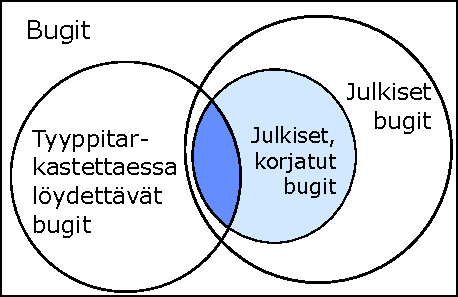
\includegraphics{images/to_type_or_not_to_type_venn.pdf}
\caption{To Type or Not to Type: Quantifying Detectable Bugs in JavaScript
         -tutkimuksen käsittelemät bugit\cite{ToTypeOrNotToType}.}
\label{fig:ToTypeOrNotToType}
\end{figure}

Kuvaajan \ref{fig:ToTypeOrNotToType} esittämässä tilanteessa suuri osa
bugeista ei ole julkisia, eli kehittäjät eivät ole havainneet bugia eivätkä
käyttäjät ole ilmoittaneet sellaisesta. Esimerkiksi seuraavanlainen koodi
saattaisi aiheuttaa vaikeasti havaittavan virheen ja jäisi helposti dynaamisessa
testaamisessa huomaamatta:

\begin{minipage}{\linewidth}
\begin{lstlisting}[caption={Vaikeasti havaittavan virheen aiheuttava koodiesimerkki}]
if (viikonpaiva === "perjantai") {
  // Alennus perjantaisin 5 euroa
  ostoskori.lisaaTuote({ nimi: "astiasto", Hinta: 10 });
} else {
  ostoskori.lisaaTuote({ nimi: "astiasto", hinta: 15 });
}
\end{lstlisting}
\end{minipage}
Esimerkin koodi ei toimi oikein perjantaisin, sillä \inlinecode{Ostos}-tyyppisen
objektin ominaisuus \inlinecode{hinta} on virheellisesti kirjoitettu isolla
alkukirjaimella. Koska bugi toistuu vain tietyissä olosuhteissa, se voi pysyä
havaitsemattomana pitkään. Staattiselle analyysille konditionaalisen ohjelman
tarkistaminen ei kuitenkaan ole ongelma ja tyyppiannotoituna kaikki kolme
työkalua pystyvätkin osoittamaan esimerkissä olevan virheen.

\section{Ohjelman optimointi käännösvaiheessa}
Aivan ensimmäiset tyyppijärjestelmät, kuten Fortranin staattinen tyypitys,
kehitettiin laskutoimitusten suoritusajan optimointia varten \cite{TypesAndProgrammingLanguages}.
Myös uudemmissa kielissä muuttujien tyypeistä saatavilla olevaa tietoa
voidaan käyttää ajonaikaisen turvallisuuden varmistavien tarkistusten
optimointiin.

Kun JavaScriptia optimoidaan käännösvaiheessa, on kuitenkin usein hyödyllistä
kiinnittää enemmän huomiota tuotetun koodin kokoon kuin suoritusaikaiseen
tehokkuuteen. Tyypillinen JavaScript-ohjelma ladataan sivulle saapuessa
internet-yhteyden yli juuri ennen suorittamista, minkä vuoksi ladattavan
koodin koon kasvattaminen minimaalisen suoritusajan edun vuoksi ei usein ole
kokonaisuudessaan hyödyllistä. Closure compiler on kehitetty erityisesti
JavaScript-koodin koon optimointia ajatellen. Muuttujanimet voidaan helposti
uudelleennimetä ilmankin staattisen tyypityksen apua, mutta sen lisäksi myös
joukko muita koodia keventäviä optimointeja on käytettävissä kun kääntäjällä
on muuttujien tyypeistä saatava tieto käytettävissä. Closure–kääntäjä osaa
uudelleennimetä myös luokkamuuttujien nimiä lyhyemmiksi, poistaa
käyttämätöntä koodia, sekä korvata yksinkertaisia funktiokutsuja siirtämällä
funktion sisältämät ohjeet kutsuntapaikalle (engl. "function inlining").

\section{Tyyppimäärittelyt dokumentaationa}
Eksplisiittisesti kirjoitetut tyypit sekä editorin antama tieto muuttujien
tyypeistä voi toimia myös aiemmin kirjoitetun koodin dokumentaationa ja
kuvauksena siitä, miten moduulia on tarkoitus käyttää. Nykyaikasten editorien
vakio-ominaisuuksiin kuuluu kirjoittamisen tukeminen automaattisilla ehdotuksilla.
Ehdotukset nopeuttavat pitkien metodinimien kirjoittamista ja toimivat
eräänlaisena dokumentaation lähteenä, sillä ohjelmoija voi tutkia luokan tai
paketin tarjoamaa sisältöä ehdotettuja nimiä selaamalla. Automaattisia ehdotuksia
on mahdollista tarjota myös dynaamisesti tyyppitarkastetuille kielille, mutta
koodipohjan kasvaessa ja muuttuessa monimutkaisemmaksi ehdotusten tarkkuus
on vaikea pitää samalla tasolla kuin staattisesti tyypitetyissä kielissä.
Huonoimmillaan ehdotetut muuttuja- ja metodinimet valitaan yksinkertaisesti
listaamalla avoimista tiedostoista löytyviä nimiä, välittämättä sen
enempää siitä onko nämä metodit määritetty juuri kyseiselle tyypille.
Edistyneemmät ehdotusmoottorit kuten Visual Studiossa käytetty IntelliSense,
suorittavat osaa JavaScript-koodista taustalla ja analysoivat siten muuttujien
tyyppejä ajonaikana \cite{PreviewingSalsa, JavaScriptIntellisense}.
Tämä tekniikka yhdistettynä tavanomaisempaan tyyppien
käännösaikaiseen päättelyyn voi riittää tarjoamaan melko kattavan kuvauksen
jonkin muuttujan tyypistä, mutta jää silti jälkeen siitä tarkkuudesta jonka
IntelliSense osaa antaa staattisesti tyypitetylle koodille.
\begin{figure}
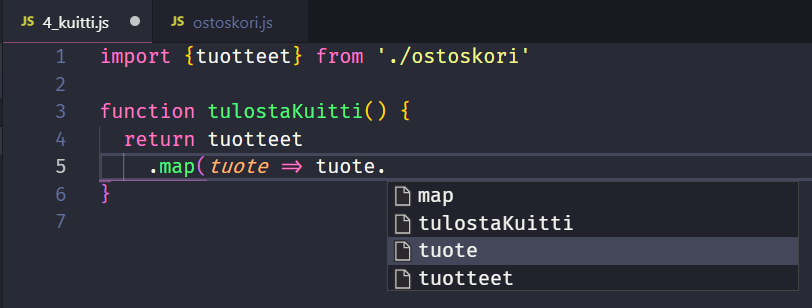
\includegraphics[width=0.8\textwidth]{images/intellisense_javascript}
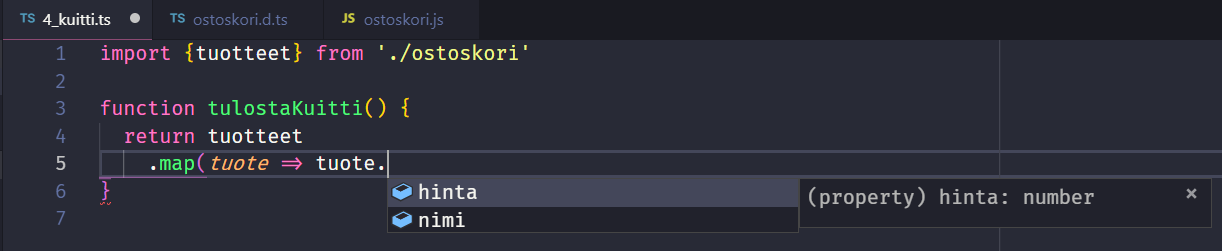
\includegraphics[width=\textwidth]{images/intellisense_typescript}
\noindent
\caption{
  IntelliSensen tarjoamat ehdotukset JavaScriptille (yllä) ja TypeScriptille (alla).
  JavaScriptille annetuissa ehdotuksissa on turhia, tiedostossa käytettyihin
  sanoihin perustuvia ehdotuksia.}
\end{figure}

Automaattisten ehdotusten vaikutuksesta ohjelmointityön tehokkuuteen ei
kuitenkaan ole yleisesti hyväksyttyä, tutkittua varmuutta. Vaikka metodien
nimet olisivatkin ohjelmoijan nähtävillä editorissa, ne eivät välttämättä
sellaisenaan tarjoa tarpeeksi hyötyä dokumentaationa jotta työtehokkuus
kasvaisi merkittävästi. Vuonna 2015 toteutettu tutkimus
``An Empirical Investigation of the Effects of Type Systems and Code Completion
on API Usability using TypeScript and JavaScript in MS Visual Studio''
testasi staattisen tyypityksen ja automaattisten ehdotusten tehokkuutta
antamalla osallistujille toteutettavaksi ohjelmointitehtävän JavaScriptillä
ja TypeScriptillä, automaattisten ehdotusten kanssa ja niitä ilman
\cite{EmpiricalInvestigationOfCodeCompletion}. Tuloksissa ei näkynyt
tilastollisesti merkittävää eroa automaattisten ehdotusten kätyön ja niiden
käyttämättä jättämisen välillä, vaikka TypeScriptiä käyttäneet suoriutuivatkin
tehtävästä muista syistä JavaScriptiä käyttäneitä tehokkaammin.